\section{Tasklet}

\begin{frame}{foreground-background}{Tasklet:die Verbindung}
 \begin{description}
  \item[foreground] der/die Interrupts
  \item[background] die normale Ausf�hrung
  \item[tasklet] Verbindung \cod{foreground} $\to$ \cod{background}
 \end{description}
\end{frame}

\begin{frame}{Tasklet}{foreground $\to$ background}
\begin{center}
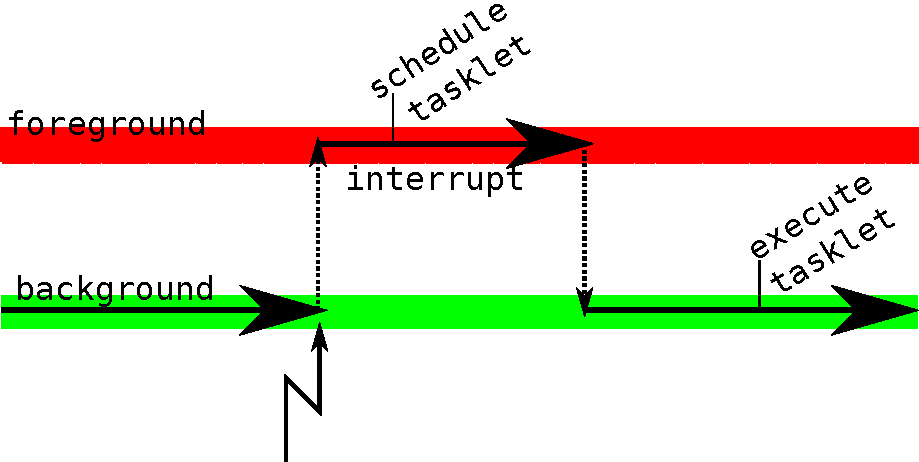
\includegraphics[width=10cm]{tasklet.pdf}
\end{center}
\end{frame}

\subsection{gpio-3.c}
\begin{frame}[fragile]{gpio-3.c}{schrittweise}
 \begin{itemize}
  \item Definition global 
       \href{https://elixir.bootlin.com/linux/latest/source/include/linux/interrupt.h\#L537}
            {\cod{tasklet\_struct}}
  \item Initialisation
       \href{https://elixir.bootlin.com/linux/latest/source/include/linux/interrupt.h\#L618}
            {\cod{tasklet\_init}}
  \item Scheduling im {\em foreground}
        \href{https://elixir.bootlin.com/linux/latest/source/include/linux/interrupt.h\#L583}
            {\cod{tasklet\_schedule}}
 \end{itemize}
 \begin{block}{Der Handler}
 \begin{lstlisting}
/* *not* called in interrupt */
static void onSWITasklet(unsigned long data)     
{
 /* do something */  
}
 \end{lstlisting}
 \end{block}
\end{frame}

